
\section{Betriebsszenarien}
\label{s:Betriebsszenarien}
Betriebsszenarien helfen die vorher beschriebene Kosten in Anwendung zu bringen und zeigen eine mögliche Entwicklung im Jahr 2050.
Für die Betriebsszenarien wurde der Flughafen Frankfurt gewählt. 
%zur besseren Veraunschaulichung
Das ist der größte Verkehrsflughafen Deutschlands und fungiert als bedeutendes Luftverkehrsdrehkreuz. 
Bei einem größeren Flughafen werden die Betriebsdifferenzen deutlicher, da das Verkehrsaufkommen wesentlich höher ist.
Der Fraport meldete im Jahr 2023 insgesamt 423764 gewerbliche Flugbewegungen, das sind im Durchschnitt 1160 Flugbewegungen pro Tag. 
Es wird angenommen, dass die Hälfte davon Abflüge sind, also müssen 580 Flugzeuge am Tag abgefertigt werden.

Die Gesamtbewegungen teilen sich nach Entfernungen folgend auf:
\begin{itemize}
    \item Kurzstrecken (bis 2500 km) sind bei 72,8 \%;
    \item Mittelstrecken (bis 6000 km) sind 9,3 \%;
    \item Langstrecken (ab 6000 km) die restlichen 17,9 \%. 
    \end{itemize}
Diese Verteilung wird auch für die Betriebsszenarien einer Flotte genutzt. 
Aufgrund der Flugeinschränkungen in der Nacht wird es angenommen, dass die Flüge von 6 bis 24 Uhr gleichmäßig stattfinden. 
Das entspricht 18 Betriebsstunden.
Wie bereits diskutiert wurde, können Kurzstrecken-Flüge durch den Einsatz von batteriebetriebenen Flugzeugen ersetzt werden. 
Es ist nennenswert, dass die Nachfrage des Kurzstrecken-Bedarfs zwar dadurch nicht gedeckt werden kann. 
In Betrachtung des tatsächlichen Flugplans sind die Spitzenstunden im Laufe des Tages zu finden, wo
der Verkehrsfluss stärker als im Durschschnitt ist. In diesem Fall werden höhere Infrastruktur- und Betriebskosten zu erwarten.
Indessen um die Interpretation zu erleichtern, wird in dieser Arbeit angenommen, dass stündlich die gleiche Anzahl an Flugzeugen 
am Flughafen abgewickelt werden. 

Für die Kurzstrecken wird zwischen Batterie-Antrieb und SAF unterschieden, 
die Mittel- und Langstrecken werden durch Flugzeuge mit Wasserstoffturbine
und SAF versorgt/erfüllt.

\subsection{Betriebsszenario I}
\begin{figure}[h]
	\centering
	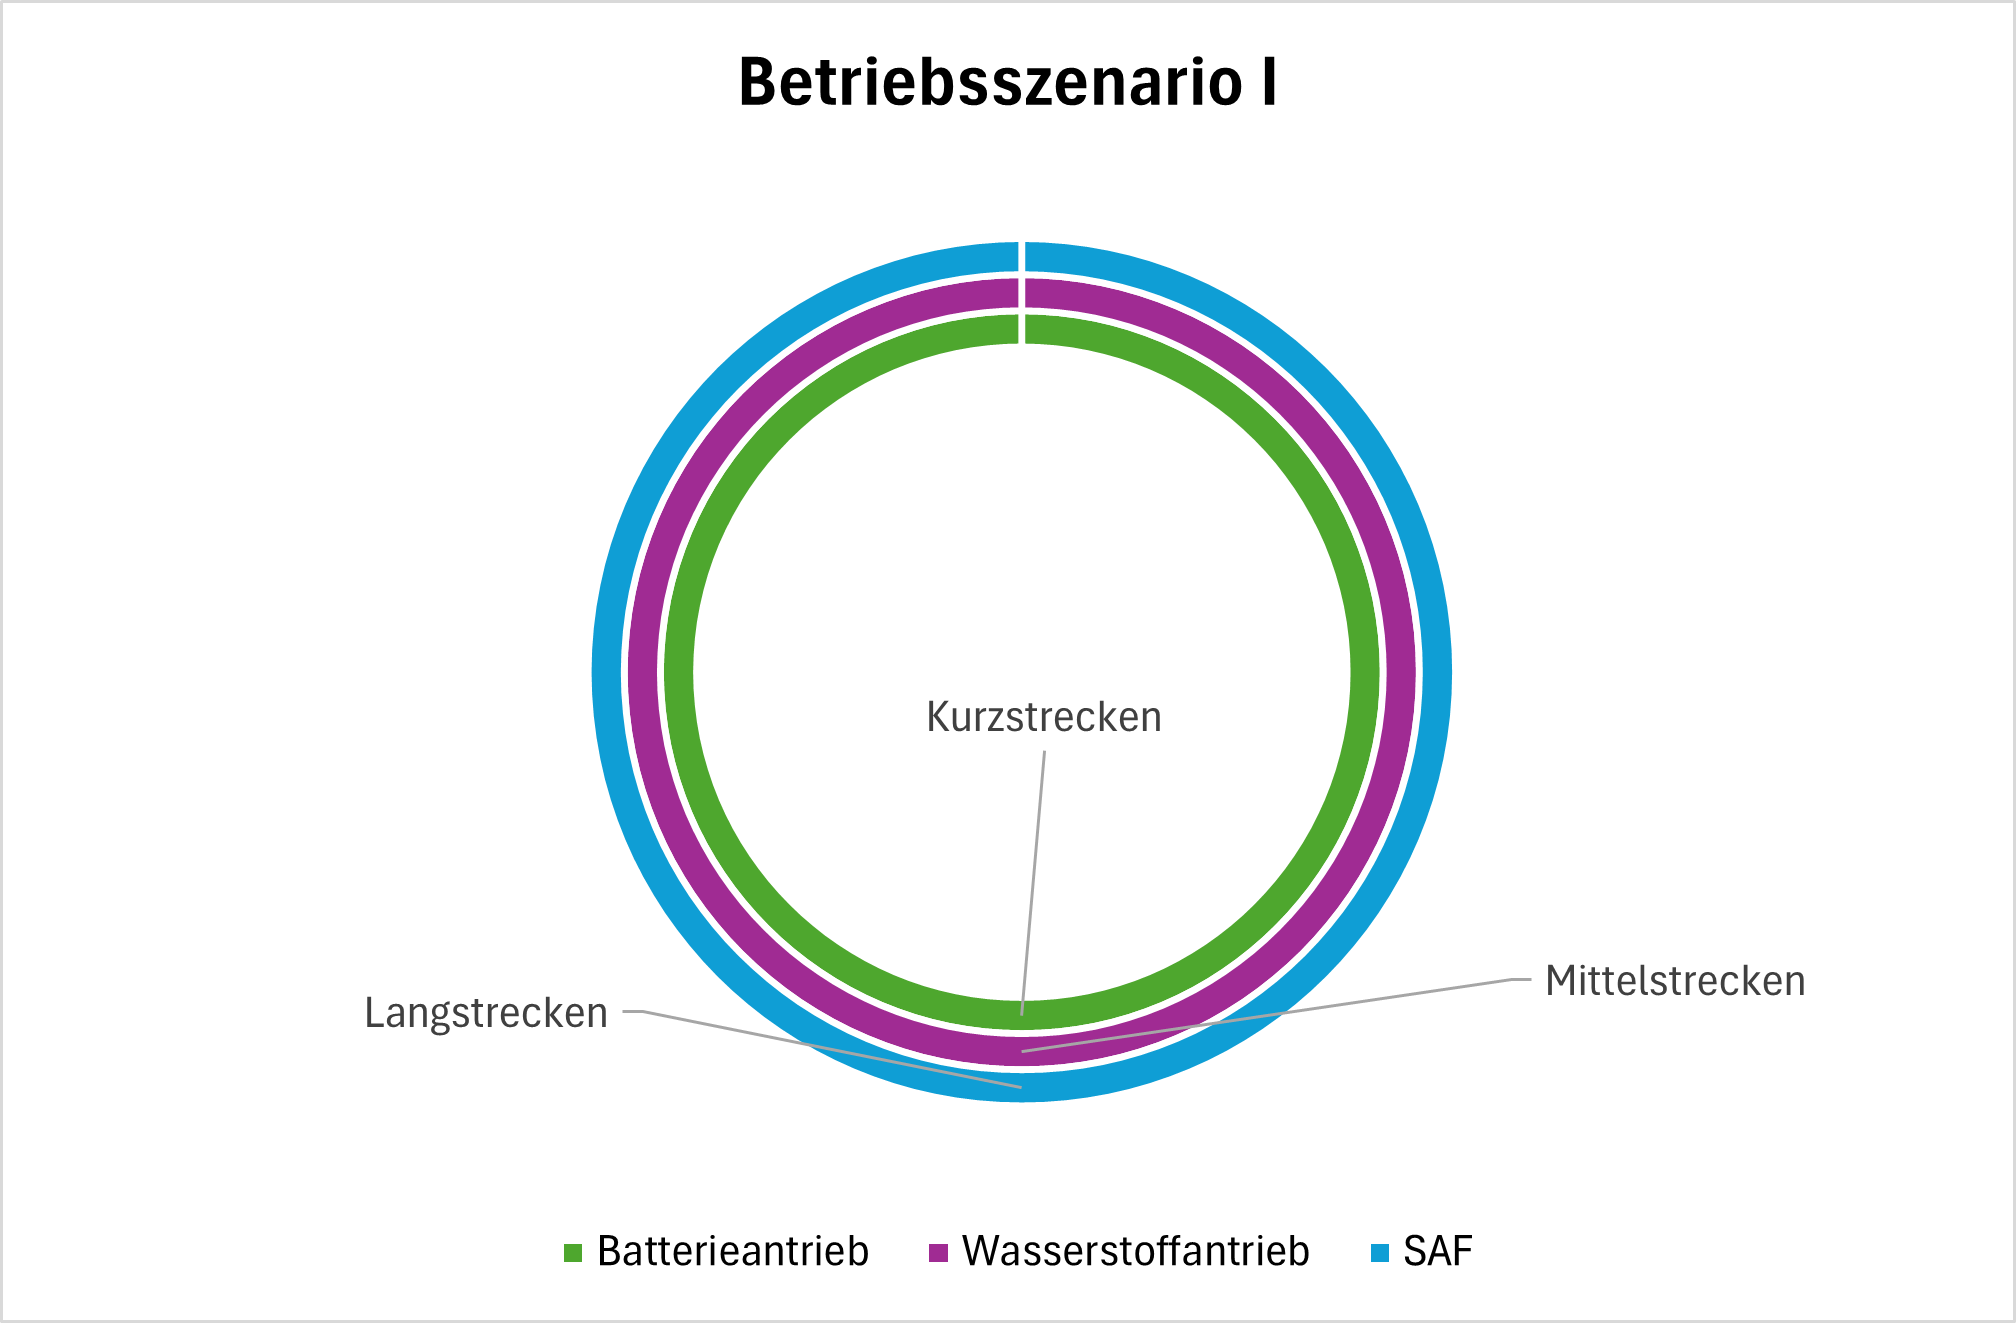
\includegraphics[width=0.8\linewidth]{Bilder/BetriebsszenarioI.png}
	\caption[Betriebsszenario I]{Aufteilung der Flugzeugflotte nach Antriebsart}
	\label{betriebsszenario1}
\end{figure}

In dem ersten Betriebsszenario wird angenommen, dass die Kurzstrecken durch die BA komplett ersetzt werden.
Die Mittelstrecken werden vollkommen durch WA und die Langstrecken durch die SAF bedient.

\subsection{Betriebsszenario II}
\begin{figure}[h]
	\centering
	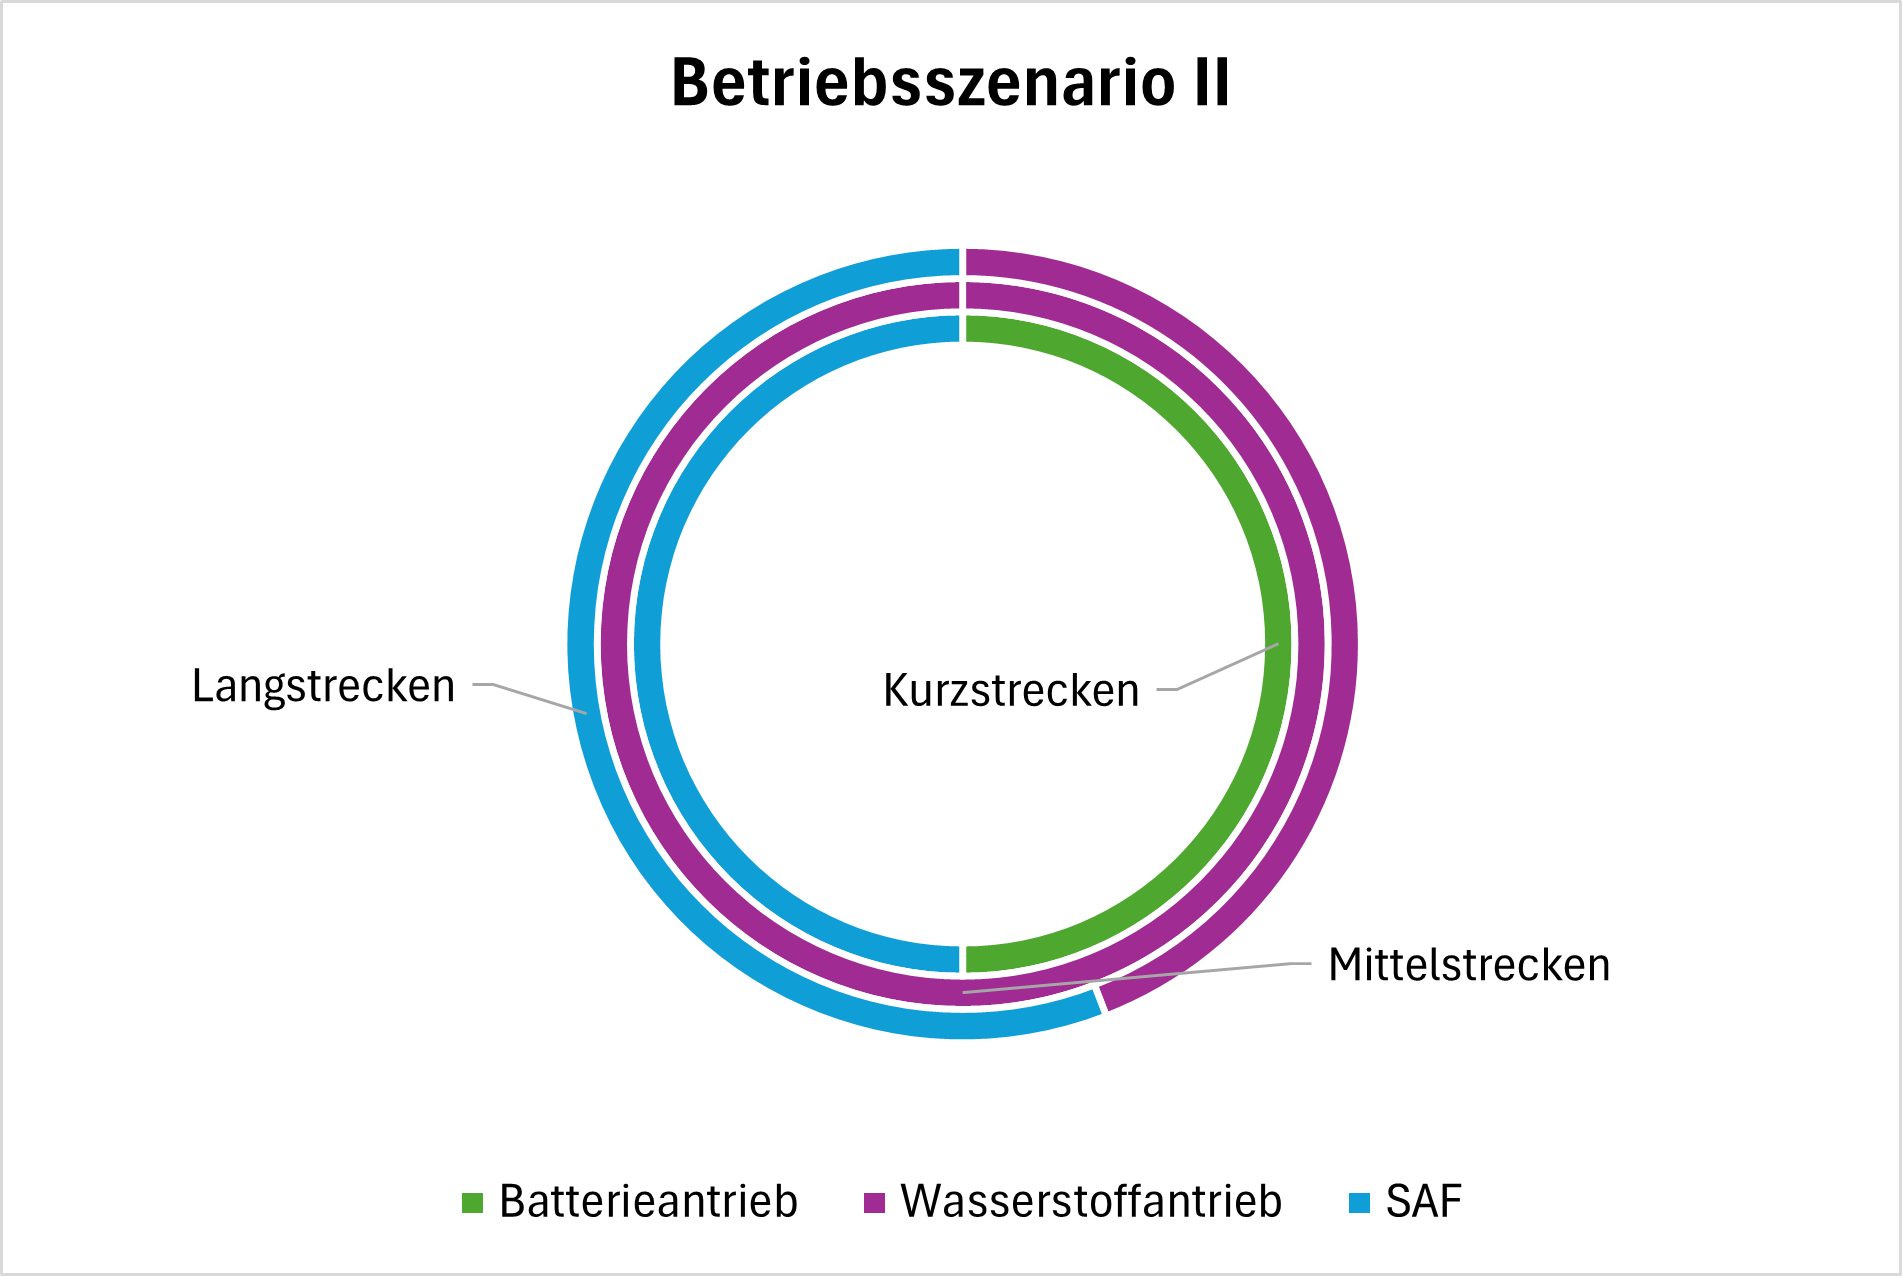
\includegraphics[width=0.8\linewidth]{Bilder/BetriebsszenarioII.png}
	\caption[Betriebsszenario II]{Aufteilung der Flugzeugflotte nach Antriebsart}
	\label{betriebsszenario2}
\end{figure}
Das zweite Betriebsszenario schlägt folgende Aufteilung vor: Die Hälfte der Kurzstrecken wird durch BA versorgt und die andere Hälfte
durch SAF; die Mittelstrecken werden genauso, wie im ersten Szenario komplett durch die Wasserstoffflugzeuge bedient und bei Langstrecken
sind 10 \% SAF und den restlichen Anteil Wasserstoff.

\subsection{Betriebsszenario III}
\begin{figure}[h]
	\centering
	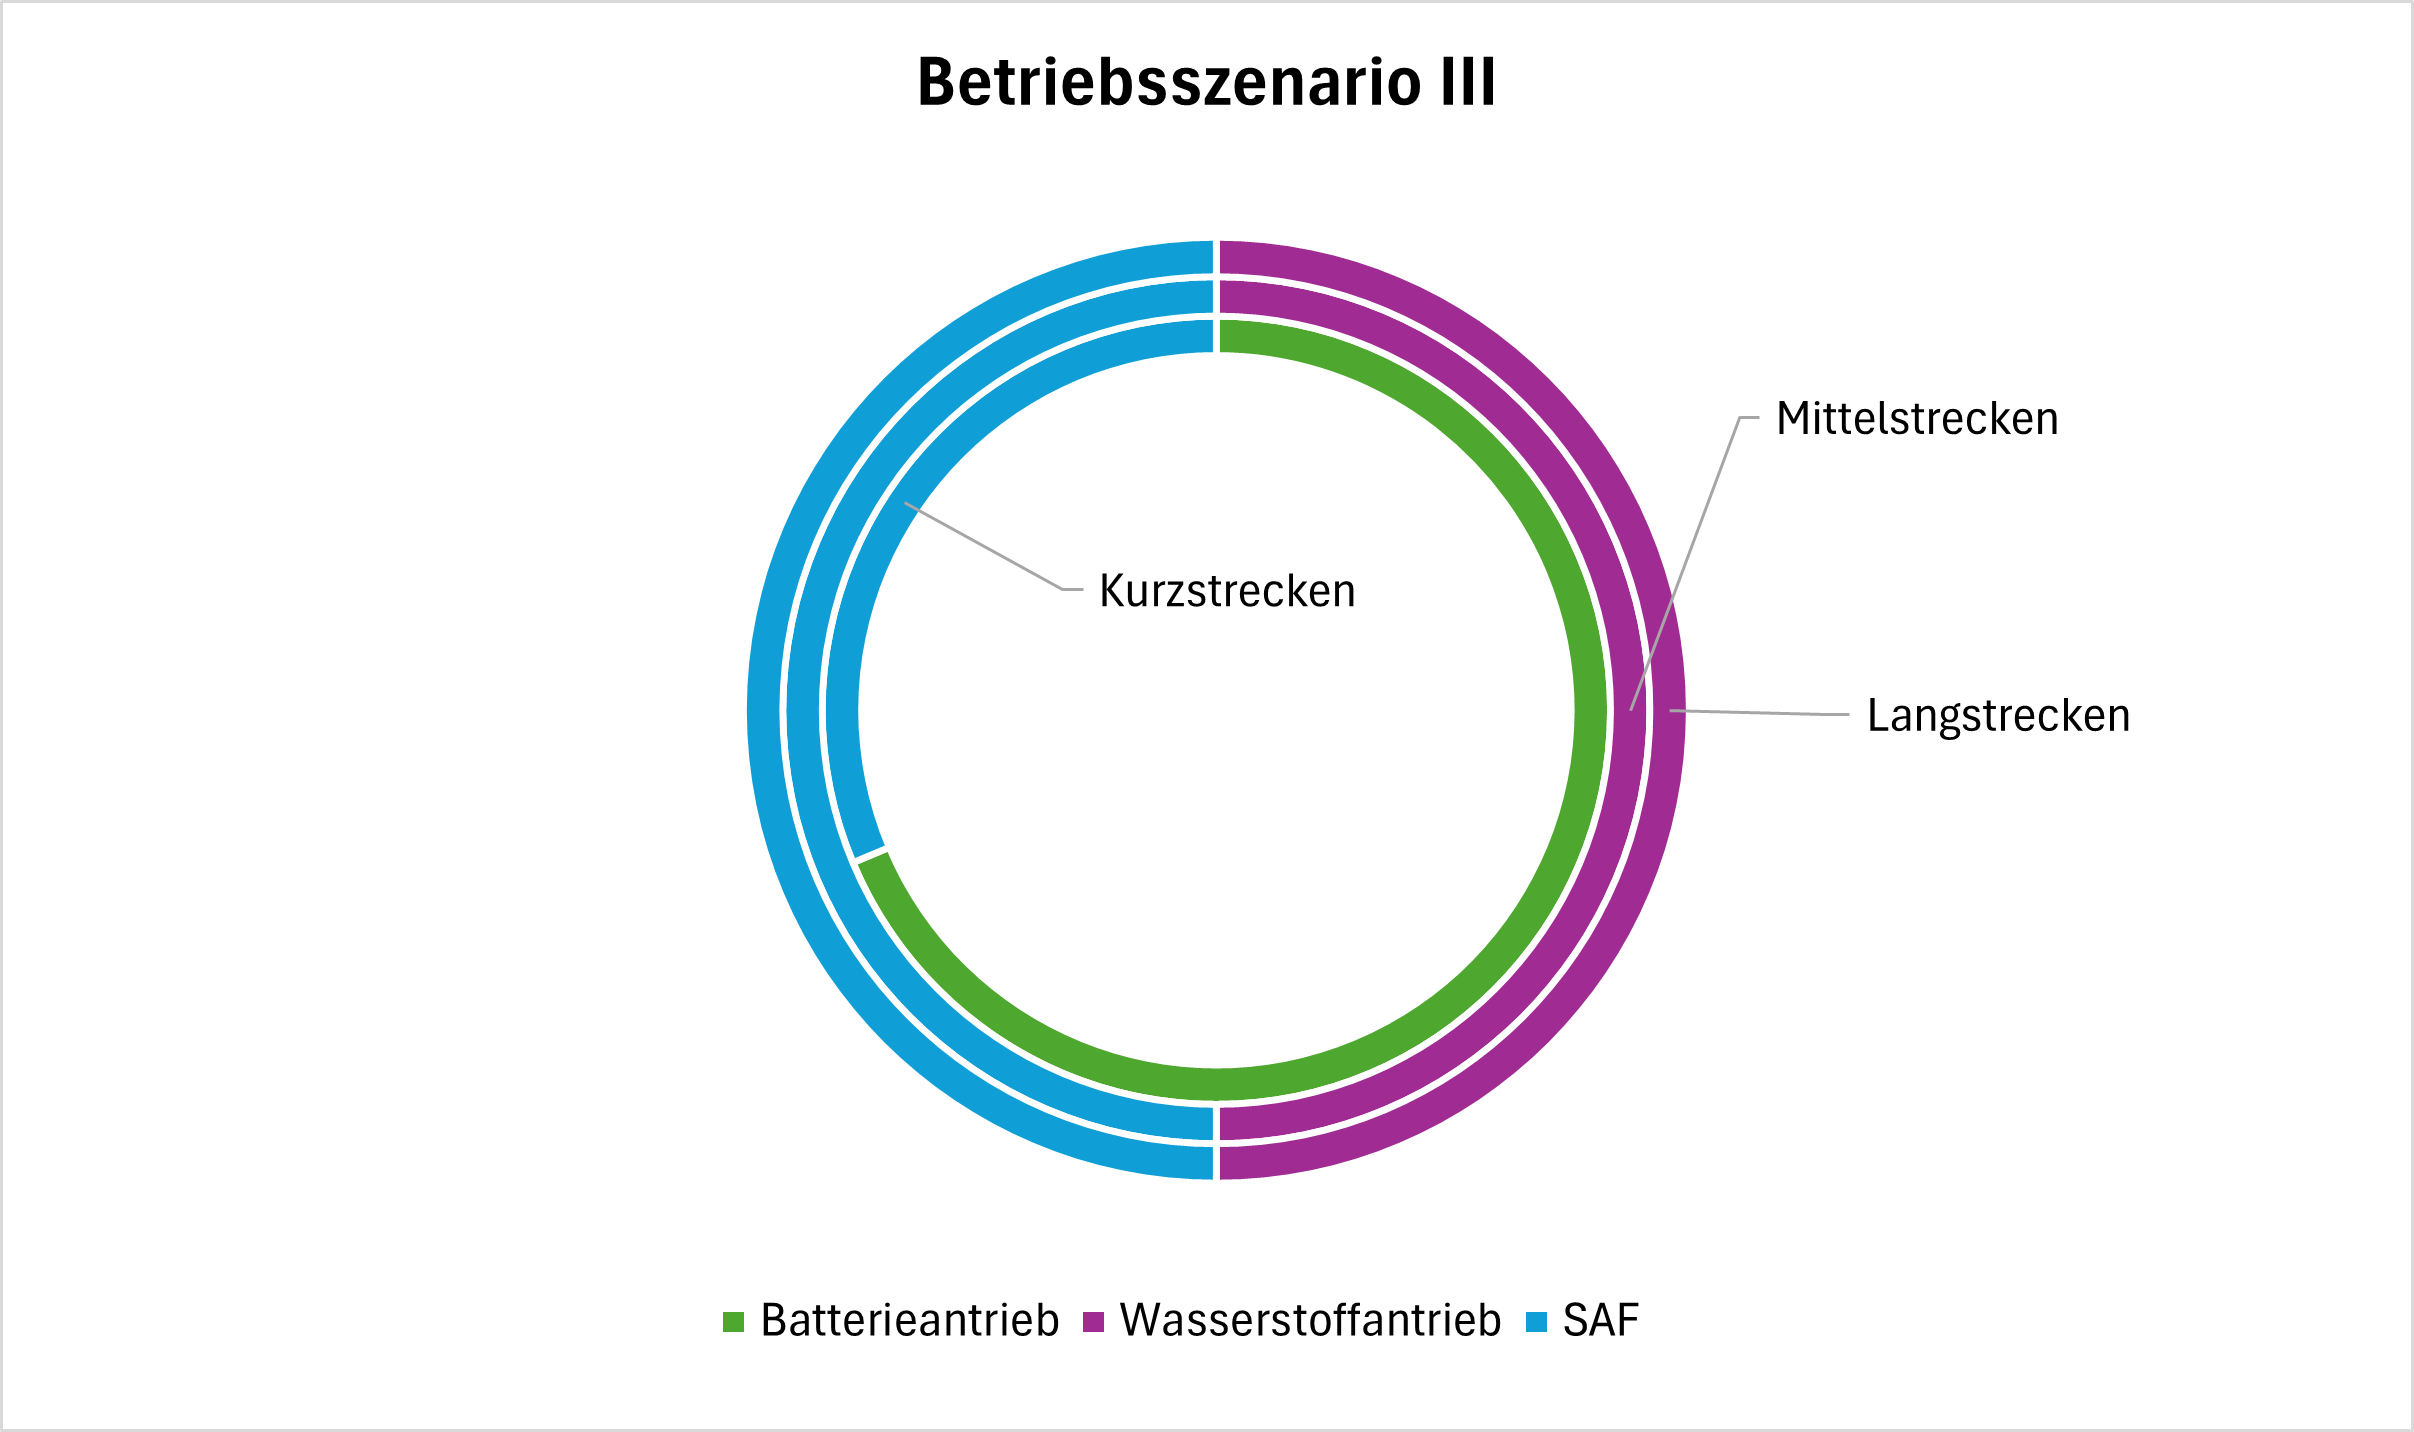
\includegraphics[width=0.8\linewidth]{Bilder/BetriebsszenarioIII.png}
	\caption[Betriebsszenario III]{Aufteilung der Flugzeugflotte nach Antriebsart}
	\label{betriebsszenario3}
\end{figure}
50 \% der Kurzstrecken sind von Batterie-Antrieb, die restlichen 22,8 \% sind mit SAF betrieben.
Mittelstrecken: die Hälfte der Mittelstrecken sind mit WA und die andere Hälfte mit SAF
Langstrecken: die Hälfte der Mittelstrecken sind mit WA und die andere Hälfte mit SAF